\chapter{Experimentación y evaluación del desempeño de la red}

\noindent
\lettrine[lines=2, lhang=0.33, loversize=0.25]{\textbf{E}}{n}\
este capítulo se detallarán los experimentos hechos con la arquitectura expuesta\
anteriormente. La metodología llevada a cabo consistió en reunir la mayor cantidad\
posible de datos para seguir con los procedimientos descritos en la Sección \ref{sec:arq-accion}.\
Los alcances de los exprimentos serán descritas más adelante, dejando en claro\
las restricciones de tiempo (para la realización de la tesis) y capacidad de equipo\
de cómputo disponible.\par
Con respecto a lo último mencionado, para los cómputos de mayor desempeño se utilizó una\
\textbf{tarjeta gráfica} (\emph{GPU}, por sus siglas en inglés) \emph{GeForce GTX 1080 Ti}\
de la marca \emph{NVIDIA}\footnote{
  Para mayor información con respecto al modelo \emph{GeForce GTX 1080 Ti},\
  consultar el sitio \url{http://la.nvidia.com/graphics-cards/geforce/pascal/la/gtx-1080-ti}.
}. Es común que en aprendizaje profundo se usen este tipo de componentes, que originalmente\
se construyen para el mundo de los videojuegos.

\section{Estructura del conjunto de datos} \label{sec:dataset}

\noindent
Como ya fue mencionado anteriormente, los datos se obtuvieron del sitio \verb+MemeGenerator.net+%
\footnote{\url{https://memegenerator.net}}.\
La información recabada en este sitio es reunida a través de usuarios alrededor del mundo,\
quienes de manera libre tienen la posibilidad de generar un nuevo meme. El sitio, además,\
agrupa a los memes en personajes (Figura \ref{meme-characters}), y los jerarquiza en base a\
su popularidad%
\footnote{
  Más aún, cualquier usuario puede crear libremente un personaje nuevo, lo que habilita la idea de\
  buscar y agrupar los memes de acuerdo a su personaje.
}.

\begin{figure}[h]
  \centering
  \begin{minipage}[l]{0.3\linewidth}
    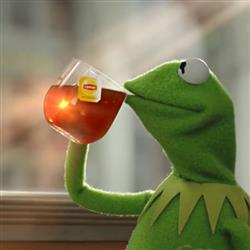
\includegraphics[width=\linewidth]{meme1}
  \end{minipage}\hfill
  \begin{minipage}[r]{0.3\linewidth}
    
\includegraphics[width=\linewidth]{meme2}
  \end{minipage}\hfill
  \begin{minipage}[r]{0.3\linewidth}
    
\includegraphics[width=\linewidth]{meme3}
  \end{minipage}
  \begin{minipage}[r]{0.3\linewidth}
    
\includegraphics[width=\linewidth]{meme4}
  \end{minipage}\hfill
  \begin{minipage}[r]{0.3\linewidth}
    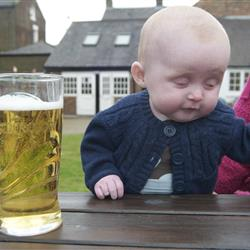
\includegraphics[width=\linewidth]{meme5}
  \end{minipage}\hfill
  \begin{minipage}[r]{0.3\linewidth}
    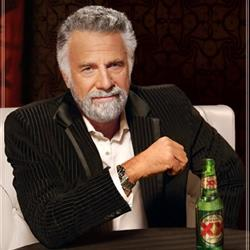
\includegraphics[width=\linewidth]{meme6}
  \end{minipage}
  \begin{minipage}[r]{0.3\linewidth}
    
\includegraphics[width=\linewidth]{meme7}
  \end{minipage}\hfill
  \begin{minipage}[r]{0.3\linewidth}
    
\includegraphics[width=\linewidth]{meme8}
  \end{minipage}\hfill
  \begin{minipage}[r]{0.3\linewidth}
    
\includegraphics[width=\linewidth]{meme9}
  \end{minipage}
  \caption{
    Ejemplos de personajes populares del sitio \url{https://memegenerator.net}.
    La mayoría de ellos gozaba de gran popularidad entre los años 2009 y 2013;
    la evolución de la viralidad de los mismos y el surgimiento de otros sitios web
    para compartir memes son algunas causas que pueden explicar su ``extinción''.
    (Tomado de \url{https://memegenerator.net}.)
  }
  \label{meme-characters}
\end{figure}

Mediante una búsqueda \emph{por profundidad}, a través del árbol de páginas web, definido por cada uno de los personajes\
del sitio, uno encuentra una gran cantidad de leyendas separadas de la imagen de su personaje asociado.\
Es decir, por cada personaje se extrae una imagen y tantas leyendas como sea posible (Figura \ref{meme-separation}).\par
Para llevar a cabo este fin, se programó un \textbf{rastreador web} (\emph{web crawler}) para llevar a cabo\
la búsqueda de la información y la acumulación de los datos. Se escribió un programa en el lenguaje de\
programación \textbf{Python} (versión 3.6)\footnote{\url{https://www.python.org}} con la biblioteca\
\textit{Scrapy} (versión 1.4.0)\footnote{\url{https://scrapy.org}}, la cual organiza hilos de ejecución concurrentes\
para obtener el contenido de las \verb+URL+'s necesarias mediante peticiones \verb+GET+ de \verb+HTTP+.\
Al final, se organizaron los datos bajo la jerarquía presente en la Figura \ref{file-hierarchy}.

\begin{figure}[h]
  \centering
  \begin{minipage}[l]{\linewidth}
    \dirtree{%
      .1 personaje-1/.
      .2 personaje-1{.}csv.
      .2 personaje-1{.}jpg.
      .2 personaje-1-metadata{.}csv.
      .1 personaje-2/.
      .2 personaje-2{.}csv.
      .2 personaje-2{.}jpg.
      .2 personaje-2-metadata{.}csv.
      .1 {.}.
      .1 {.}.
      .1 {.}.
      .1 personaje-n/.
      .2 personaje-n{.}csv.
      .2 personaje-n{.}jpg.
      .2 personaje-n-metadata{.}csv.
    }
  \end{minipage}
  \caption{
    Como se observa, los datos se guardaron bajo el formato \texttt{CSV}, asociando cada leyenda con la \texttt{URL}
    de su meme asociado y su idioma de origen (Figura \ref{meme-file}). Se estima que un $90\%$ de datos está en inglés.
  }
  \label{file-hierarchy}
\end{figure}

\begin{figure}[H]
  \centering
  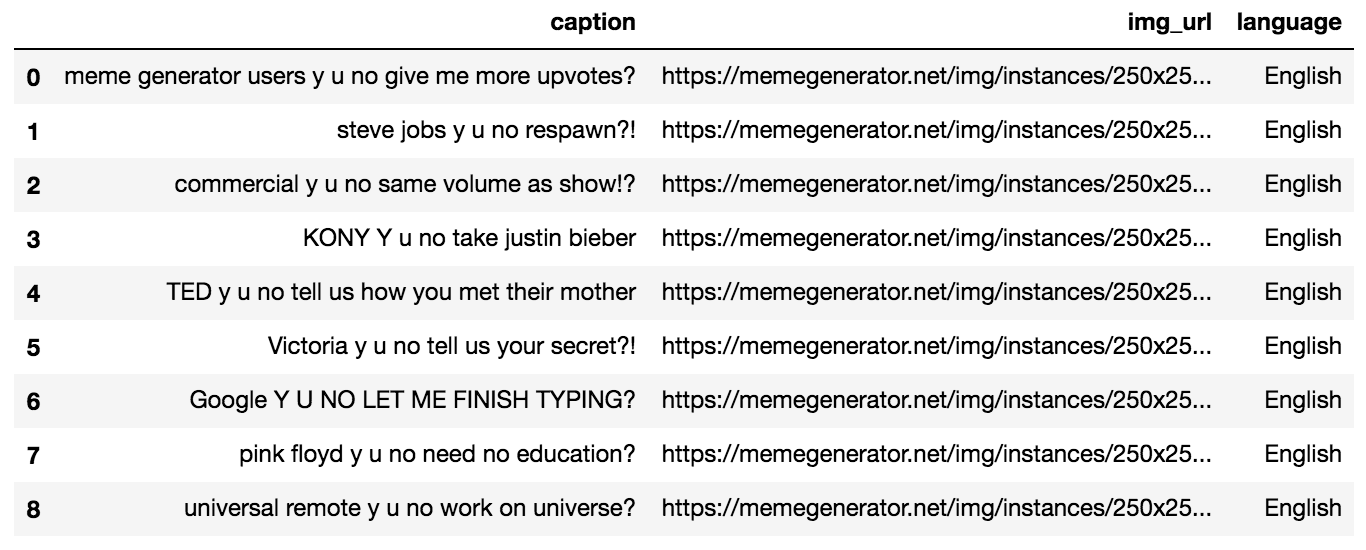
\includegraphics[width=\textwidth]{meme-file}
  \caption{
    De esta manera se guardaron cada una de las leyendas de cada personaje.
  }
  \label{meme-file}
\end{figure}

\begin{figure}
  \centering
  \begin{minipage}[l]{\linewidth}
    
\includegraphics[width=\linewidth]{thesis-i-demand-trial-by-combat}
  \end{minipage}\hfill
  \begin{minipage}[r]{0.5\linewidth}
    
\includegraphics[width=\linewidth]{tyrionlannister}
  \end{minipage}\hfill
  \begin{minipage}[r]{0.5\linewidth}
    \verb+thesis  i demand trial by combat+
  \end{minipage}
  \caption{
    La ilustración de la parte superior constituye a un meme que integra a un personaje con su leyenda y
    es el objeto que se propaga a través de Internet. Los datos que se reunieron se separaron como se
    indica en la ilustración de la parte inferior.
    (Tomado de \url{https://memegenerator.net}.)
  }
  \label{meme-separation}
\end{figure}

\section{Experimentos}

\noindent
Los experimentos realizados obedecen a lo sugerido por la teoría presentada en los dos capítulos anteriores.\
Se buscó seguir la metodología sugerida por el \emph{estado del arte} (\cite{DBLP:journals/corr/VinyalsTBE16}).\
Por ello, se eligió trabajar con el lenguaje de programación Python (versión 3.6) y las bibliotecas\
\textbf{Tensorflow} (versión 1.3.0)\footnote{\url{https://www.tensorflow.org}} y \textbf{Keras}\
(versión 2.0.8)\footnote{\url{https://keras.io}}.\par
Ambas bibliotecas son obra \emph{reciente} de la división de código abierto de \emph{Google}.\
\emph{Tensorflow} surgió como una iniciativa para compartir la manera en que dicha empresa despliega\
sus proyectos que involucran aprendizaje profundo. El paradigma que se sigue consiste en definir un\
grafo dirigido de \emph{tensores} como nodos, en el cual fluirá la información\footnote{
  En cada nodo del grafo, se definen \emph{operaciones} (lectura y escritura de archivos, operaciones\
  matriciales, etc.) y se da la posibilidad de especificar si van a correr en un GPU, si se cuenta con uno.
}; acto seguido, se ``compila'' el modelo y se levanta una sesión para ejecutarlo. Así, \emph{Tensorflow}\
utiliza la sintaxis de \emph{Python} para construir redes neuronales en un mayor nivel.\par
Por otro lado, \emph{Keras} se define a sí misma como una interfaz de programación de aplicaciones (\emph{API})\
de alto nivel, que utiliza como motor de ejecución a \emph{Tensorflow}. Es decir, el programador es capaz\
de escribir código que defina una red neuronal y se ejecute secuencialmente. \emph{Keras}, además,\
facilita la tarea de definir un modelo profundo con una sintaxis más amigable que la de \emph{Tensorflow}\
y configura algunos \emph{hiper-parámetros} de ésta, con el fin de facilitar el prototipado de redes neuronales\
profundas.

\subsection{El \emph{primer} experimento}

\noindent
Vinyals, \emph{et al}, presentan tanto en \cite{DBLP:journals/corr/VinyalsTBE14} como en \cite{DBLP:journals/corr/VinyalsTBE16}\
el \emph{estado del arte} de los modelos neuronales capaces de generar descripciones a partir de imágenes.\
Por ende, el primer paso experimental consistió en replicar el entrenamiento completo, usando el conjunto de datos\
\emph{ImageNet}.

\begin{experiment} \label{experiment:1}
  Utilizando pesos pre-entrenados%
  \footnote{
    \emph{Tensorflow} provee un conjunto de modelos previamente entrenados bajo un subconjunto de\
    \emph{ImageNet} (\url{http://www.image-net.org/challenges/LSVRC/2012/}). Esto ahorra tiempo en la vectorización\
    de imágenes. Para mayor información, consultar el sitio\
    \url{https://github.com/tensorflow/models/tree/master/research/slim\#tensorflow-slim-image-classification-library}.
  } de Inception V3, se realizó el proceso de generar un tensor de incrustaciones de las imágenes de ImageNet\
  en un espacio vectorial. Acto seguido se alimentó una LSTM con dicho tensor, como memoria inicial, y se\
  entrenó utilizando las leyendas asociadas a cada imagen.
\end{experiment}

Dentro de las ventajas consecuentes del Experimento \ref{experiment:1}, está el tener una implementación\
de una LSTM para ser entrenada de nuevo, con cualquier memoria inicial. El desempeño del entrenamiento\
se ilustra en la Figura \ref{exp1}. Es importante destacar que, dadas las altas dimensiones con las que\
se trabaja en cada capa, se estima que se requieren alrededor de 1 millón de épocas para que el error\
dado por la entropía cruzada se estabilice en un valor mínimo.

\begin{figure}[H]
  \centering
  \begin{minipage}[c]{\linewidth}
    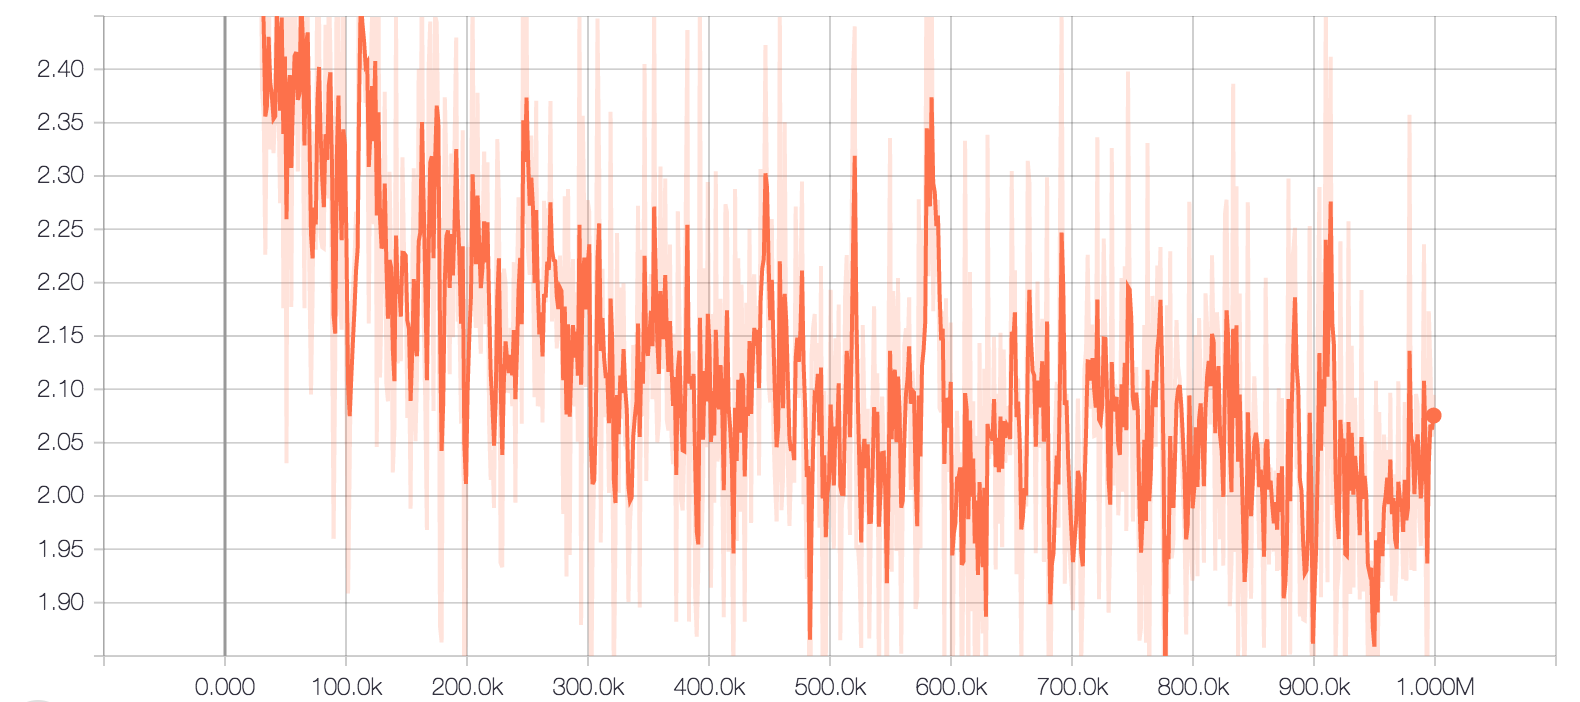
\includegraphics[width=\linewidth]{exp1-1}
  \end{minipage}\hfill
  \begin{minipage}[c]{\linewidth}
    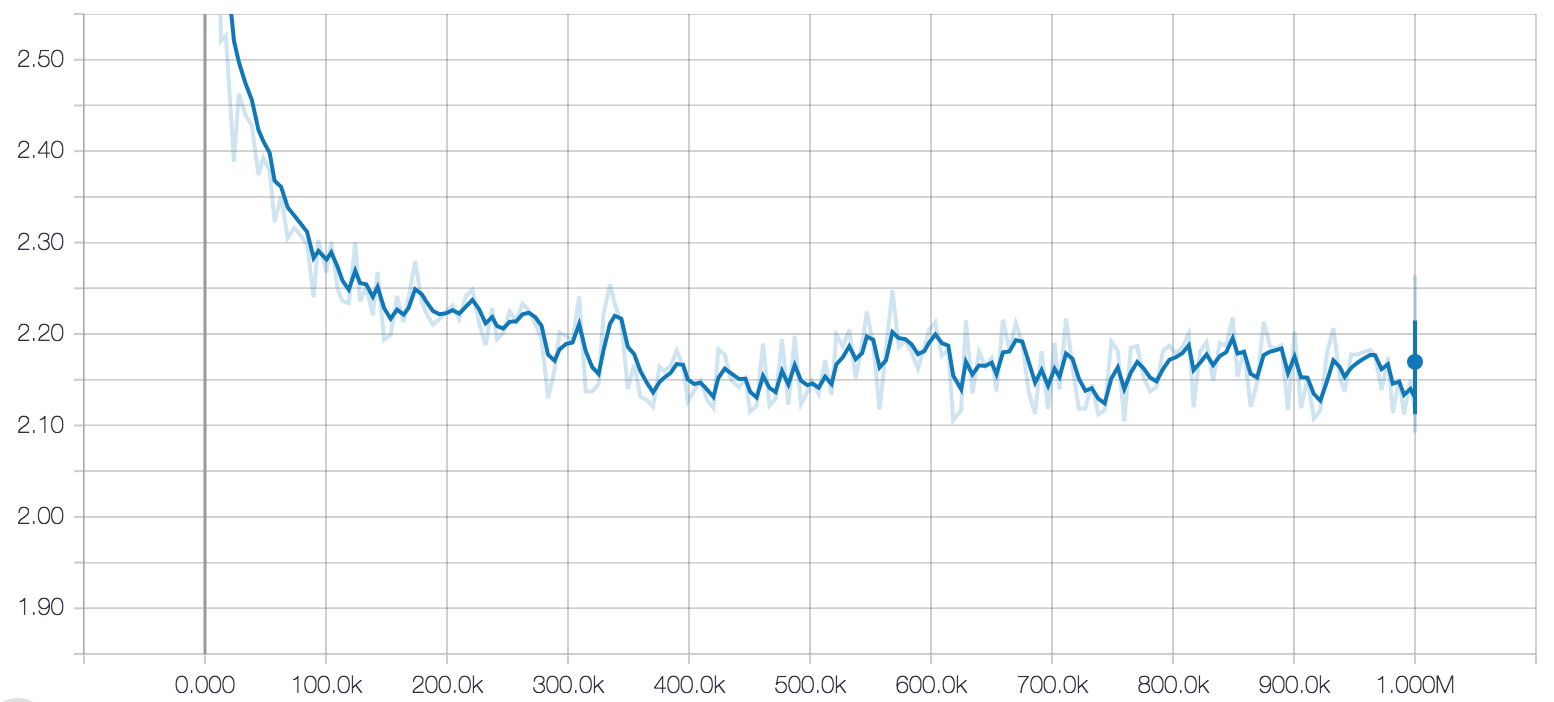
\includegraphics[width=\linewidth]{exp1-2}
  \end{minipage}
  \caption{
    De esta manera se ve la función de el error por entropía cruzada asociado al modelo del
    Experimento \ref{experiment:1}. En el gráfico de la parte superior se muestra el error
    a través de cada época del entrenamiento, mientras que el de la parte inferior se
    calculó por medio de un conjunto de datos de validación (de menor tamaño que el de entrenamiento).
    (Fuente: elaboración propia.)
  }
  \label{exp1}
\end{figure}


\subsection{Afinación de \emph{Inception V3}}

\noindent
Para aprovechar la especialización que posee \emph{Inception V3}, de reconocer patrones simples en\
imágenes, afinamos dicho modelo con un clasificador de memes. Dado que el conjunto de datos\
presentado en la Sección \ref{sec:dataset} no está dividido en ``categorías'' de memes, resulta difícil\
realizar una tarea de aprendizaje supervisado con una CNN.\par
Por otro lado, dadas las características de las imágenes de los memes, existe un patrón más o menos definido\
(rostro del personaje centrado en la imagen) que puede ser explotado contra la tarea general de aprender\
a clasificar \emph{ImageNet}. Esto nos brindó la solución para poder afinar a \emph{Inception V3}: colocar\
una capa MLP, al final de la red, con salida de dos dimensiones para decidir si la entrada es, o no es,\
un meme.\par
Las imágenes \emph{``no memes''} utilizadas en este punto se tomaron aleatoriamente muestreando alrededor\
de 4 mil ejemplares de \emph{ImageNet}. Se trabajó bajo la premisa de que la profundidad de la red\
alcanzará para generalizar la identificación de las características presentes en un meme. Después de todo,\
nuestro conjunto de datos posee imágenes de mucho menor complejidad que las existentes en \emph{Inception V3}.

\begin{experiment} \label{experiment:2}
  Afinación de Inception V3, entrenando un clasificador entre lo que es un meme y lo que no es. Se quita\
  la última capa y se añade un MLP con dos dimensiones de salida. El desempeño de este experimento\
  se ilustra en la Figura \ref{exp2}.
\end{experiment}

\begin{figure}[H]
  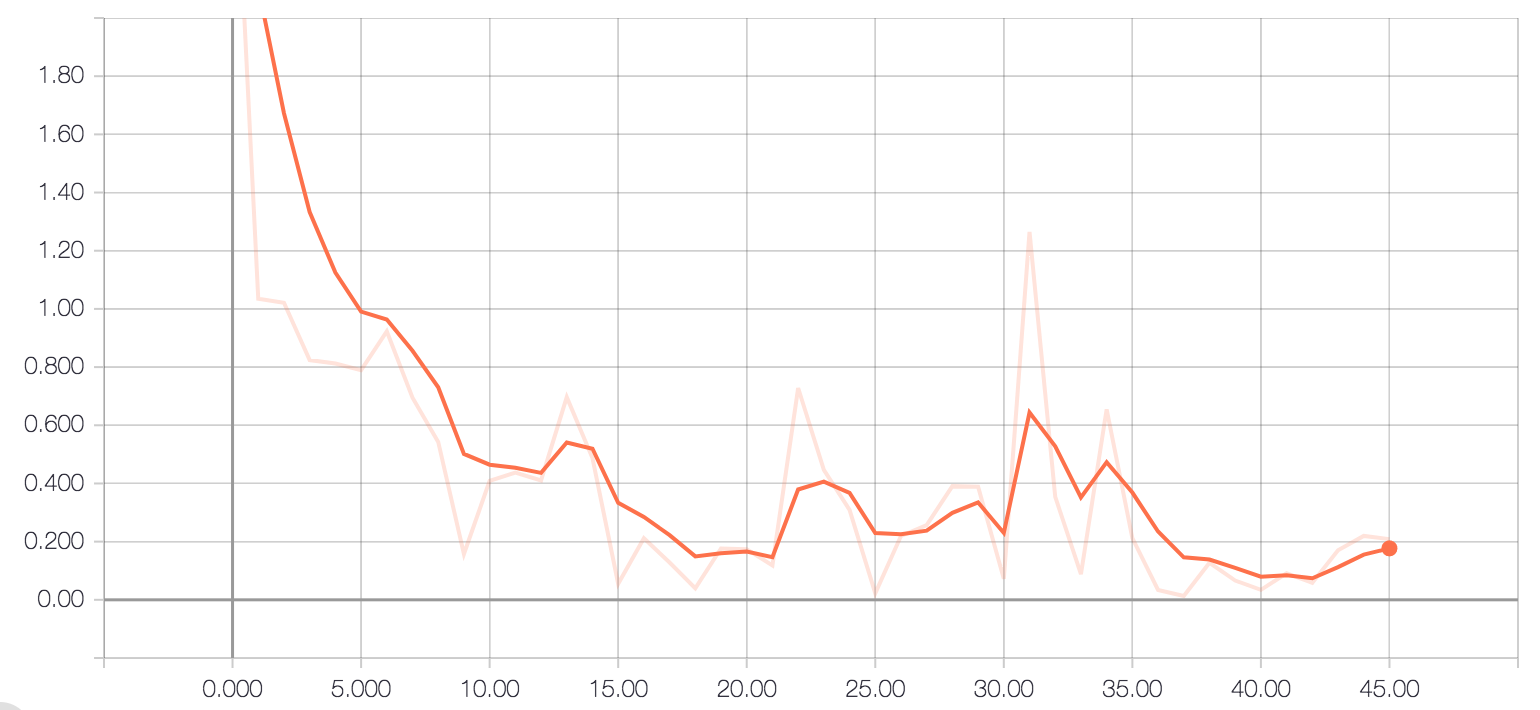
\includegraphics[width=\linewidth]{exp2-1}
  \caption{
    Función de error para el Experimento \ref{experiment:2}.
    (Fuente: elaboración propia.)
  }
  \label{exp2}
\end{figure}

\subsection{Una red convolucional \emph{pequeña}}

\noindent
Aunque afinar una CNN profunda, previamente entrenada, es un procedimiento justificado por la literatura,\
el número máximo de imágenes que conforman el conjunto de datos sugiere otro tratamiento.\
En total se tienen 4379 personajes, de los cuales se suele tomar un $80\%$ para entrenamiento y el resto\
para validación. Esto indica que entrenar una red neuronal desde cero no es una mala apuesta,\
después de todo, de acuerdo a \cite{DBLP:journals/corr/YosinskiCBL14}.

\begin{experiment} \label{experiment:3}
  Se entrenó una red neuronal \emph{bastante menos profunda} a \emph{Inception V3}. Se usaron\
  los mismos datos que para la afinación descrita en el Experimento \ref{experiment:2}.\
  La arquitectura de esta red se muestra en la Tabla \ref{capas-small}, mientras que\
  el desempeño del entrenamiento se ilustra en la Figura \ref{exp3}.
\end{experiment}

\begin{table}[H]
  \resizebox{\textwidth}{!}{
    \begin{tabular}{|l|c|c|}
      \hline
      \textbf{tipo} & \textbf{tamaño de filtro} & \textbf{número de filtros}\\
      \hline \hline
      CONV & $3 \times 3$ & $32$ \\
      \hline
      CONV & $3 \times 3$ & $16$ \\
      \hline
      POOL & $2 \times 2$ & - \\
      \hline
      DROPOUT & $25\%$ de las neuronas se ignoran & - \\
      \hline
      MLP & $128$ unidades de salida & - \\
      \hline
      DROPOUT & $50\%$ de las neuronas se ignoran & - \\
      \hline
      MLP & $2$ unidades de salida & - \\
      \hline
    \end{tabular}
  }
  \caption[Nota al pie]{
    Arquitectura utilizada para el Experimento \ref{experiment:3}. Las capas
    \textbf{DROPOUT} constituyen una popular técnica de \emph{regularización}\footnotemark en
    la que se descarta un porcentaje dado de las neuronas de entrada con el fin
    de evitar un sobreajuste sobre el conjunto de datos en cuestión.
  }
  \label{capas-small}
\end{table}

\footnotetext{
  Las técnicas de \textbf{regularización}, en aprendizaje automático, añaden una
  restricción adicional al problema en cuestión para provocar que los valores
  del modelo propuesto se ajusten completamente al conjunto de datos de entrenamiento.
  Es decir, evitar el \emph{sobreajuste} y favorecer la generalización hacia datos
  no observados durante el entrenamiento.
}

\begin{figure}[H]
  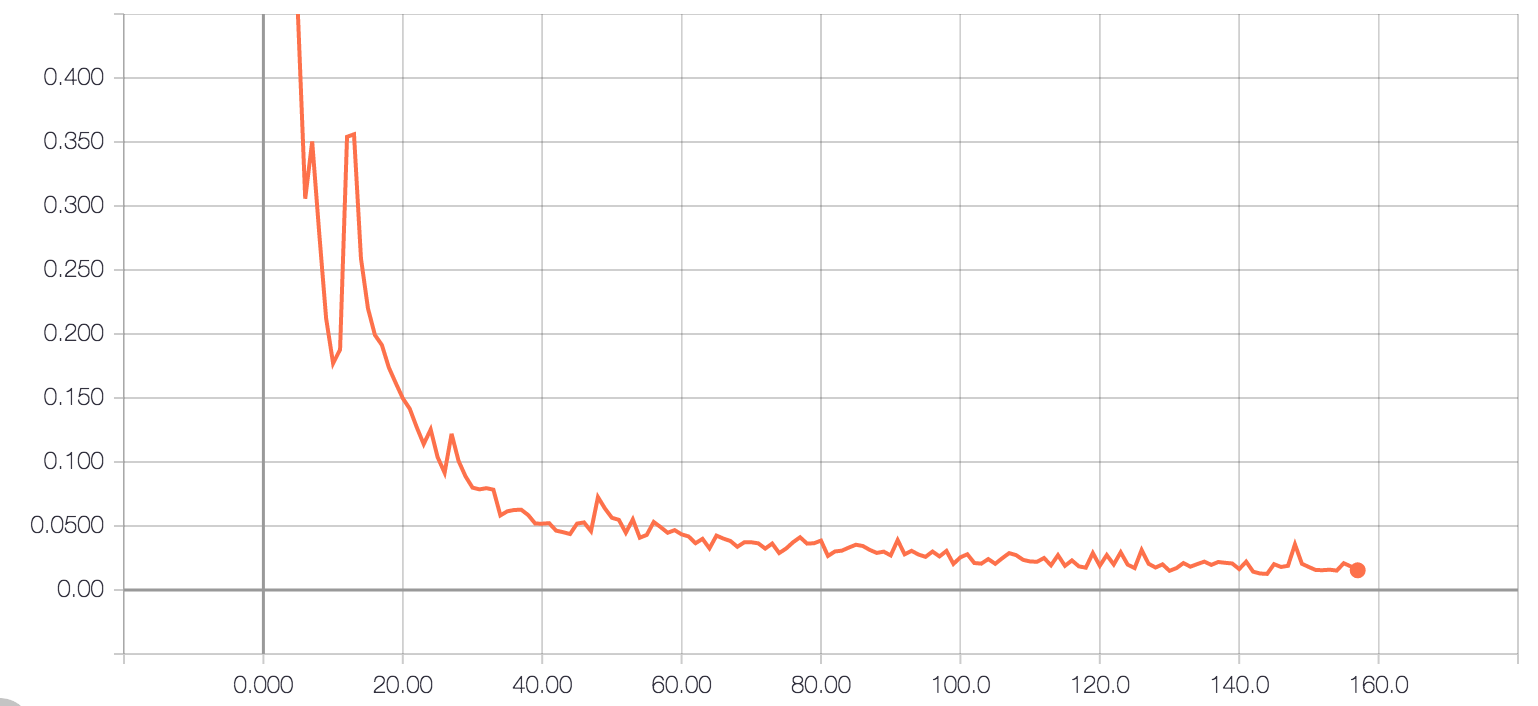
\includegraphics[width=\linewidth]{exp3-1}
  \caption{
    Función de error para el Experimento \ref{experiment:3}. Obsérvese que
    solo se requirieron alrededor de 150 épocas de entrenamiento para llegar a un
    valor óptimo; esto dado el tamaño del conjunto de datos (\emph{memes} y
    \emph{no memes}) que es bastantes órdenes de magnitud más pequeño el\
    conjunto de datos de entrenamiento presentado en la Sección \ref{sec:dataset}.
    (Fuente: elaboración propia.)
  }
  \label{exp3}
\end{figure}

\subsection{Entrenamiento de la LSTM}

\noindent
Teniendo en cuenta las maneras de obtener los \emph{códigos convolucionales} para las imágenes\
del conjunto de datos de memes, lo que procede es entrenar la LSTM con la correspondiente\
memoria inicial. A continuación, se listan diversos experimentos junto con una explicación\
de lo que motivó a llevarse a cabo, así como un breve análisis \emph{empírico} de los resultados obtenidos.\par
Además, se dan detalles sobre si se hizo algún procesamiento previo de las leyendas de entrenamiento y\
el vocabulario. En tareas que involucran procesamiento de algún \emph{corpus lingüístico}, es\
común que se trabaje solamente con palabras en minúsculas, así como la supresión de palabras\
con un bajo número de frecuencias en el conjunto de datos. En este último caso, se suelen reemplazar\
dichas palabras por un \emph{token} que indique la imposibilidad de su reconocimiento\
(\verb+<UNK>+, por ejemplo).

\begin{experiment} \label{experiment:4}
  Utilizando únicamente 97 personajes, cada uno con un promedio de 700 leyendas, se entrenó\
  una LSTM sin restricción del vocabulario. Es decir, no se hizo procesamiento previo alguno sobre\
  las leyendas; por ende, el vocabulario construído tuvo alrededor de 20 mil palabras distintas.\
  Además, se utilizó como CNN a la \emph{Inception V3} sin ser afinada, con los pesos previamente\
  entrenados sobre \emph{ImageNet}.\par
  El desempeño fue deficiente tanto en entrenamiento (Figura \ref{exp4}) como en los resultados.\
  Las siguientes observaciones fueron notables:
  \begin{itemize}
  \item los códigos convolucionales resultantes del paso por la CNN fueron indistinguibles entre\
    una imagen y otra, dejando en claro la necesidad de realizar una afinación);
  \item lo anterior provocó que las leyendas fueran todas iguales para imágenes distintas.
  \end{itemize}
\end{experiment}

\begin{figure}[h]
  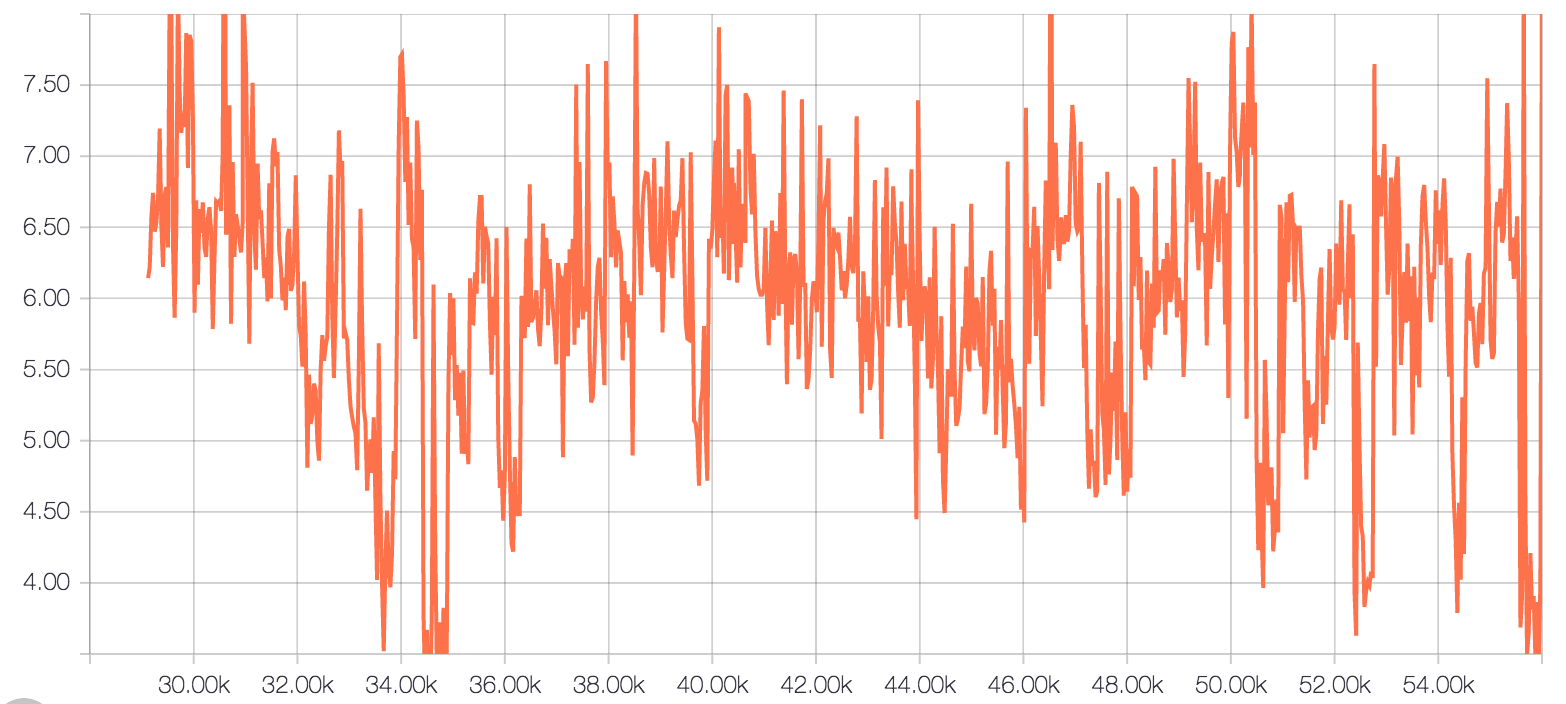
\includegraphics[width=\linewidth]{exp4-1}
  \caption{
    Función de error para el Experimento \ref{experiment:4}.
    (Fuente: elaboración propia.)
  }
  \label{exp4}
\end{figure}

\begin{experiment} \label{experiment:5}
  Se usaron los mismos datos que los que se usaron para el Experimento \ref{experiment:4} pero\
  con la \emph{Inception V3} previamente afinada. Esto provocó que entre cualesquiera\
  dos imágenes diferentes, existieran dos códigos convolucionales con valores suficientemente\
  distintos; lo que implica que las leyendas generadas serán también distintas.\par
  El tensor de imágenes y leyendas de entrada $(I, S)$ se fue construyendo en orden,\
  de manera que todas las leyendas de un solo personaje permanecían en posiciones contiguas.\
  Dada la cantidad desmedida de leyendas, esto provocó que tras ciertas iteraciones se sobreentrenara\
  el modelo sobre un mismo lote. Así, al probar el modo de \verb+inferencia+ del mismo,\
  se podía observar claramente una tendencia por repetir la ``manera de hablar'' de un cierto personaje.\
  Iteraciones más tarde, esto cambiaba para que el modelo comenzará a repetir la manera de\
  hablar de otro personaje. Una de las evidencias del sobreajuste se ilustra en la Figura \ref{exp5}.
\end{experiment}

\begin{figure}[h]
  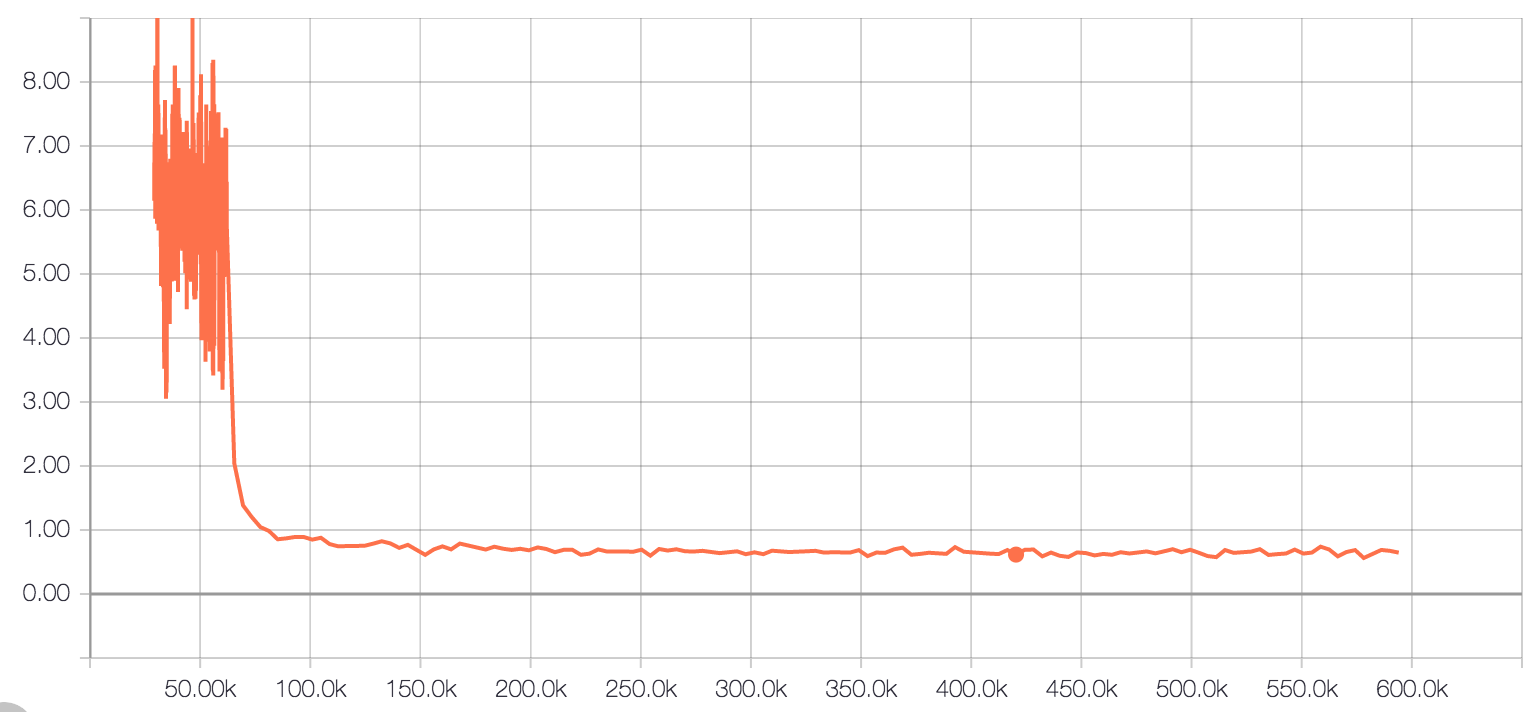
\includegraphics[width=\linewidth]{exp5-1}
  \caption{
    Función de error para el Experimento \ref{experiment:5}.
    (Fuente: elaboración propia.)
  }
  \label{exp5}
\end{figure}

\begin{experiment} \label{experiment:6}
  Aquí se usaron alrededor de 3 mil personajes, eliminando todas las palabras que no aparezcan al menos\
  5 veces en todo el conjunto de datos. Además, se mezclaron los datos de manera aleatoria en el\
  tensor $(I, S)$; esto provocó la diversificación en la manera con la que se generan leyendas para\
  imágenes que no aparecen en el conjunto de entrenamiento. Más aún, se usaron únicamente 5 leyendas\
  para cada personaje, los cuales fueron procesados por la \emph{Inception V3} afinada. El desempeño\
  convergió de la manera ilustrada en la Figura \ref{exp6}.
\end{experiment}

\begin{figure}[H]
  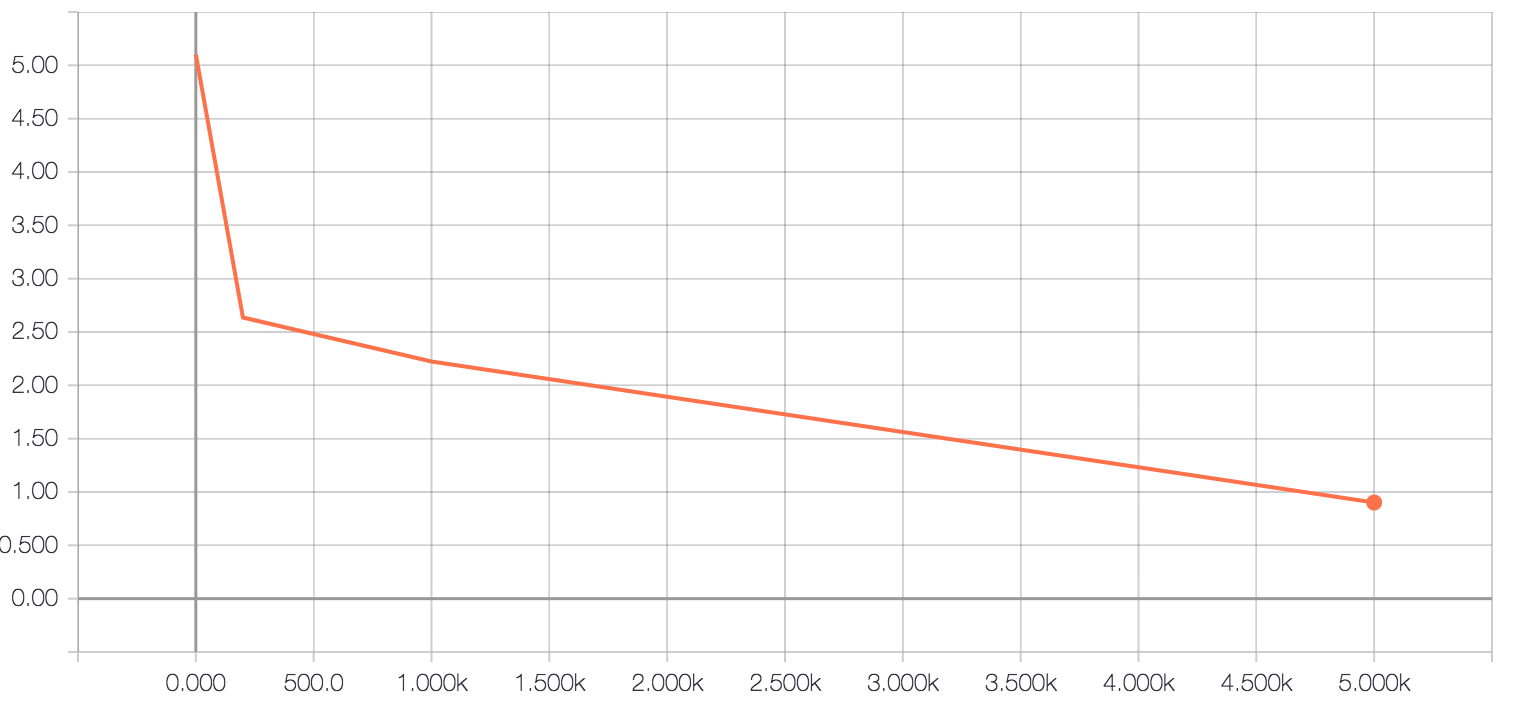
\includegraphics[width=\linewidth]{exp6-1}
  \caption{
    Función de error para el Experimento \ref{experiment:6}.
    NOTA: ESTA IMAGEN DEBE SER ACTUALIZADA.
    (Fuente: elaboración propia.)
  }
  \label{exp6}
\end{figure}


\begin{experiment} \label{experiment:7}
  Este experimento fue idéntico al Experimento \ref{experiment:6}; sin embargo, se utilizó la CNN pequeña\
  descrita en el Experimento \ref{experiment:3}. El entrenamiento arrojado fue muy similar a lo obtenido\
  en el Experimento \ref{experiment:6} (Figura \ref{exp7}); no obstante, se buscaba mejorar la calidad de las leyendas\
  generadas, algo que se logró sin ser una gran mejora empírica.
\end{experiment}

\begin{figure}[h]
  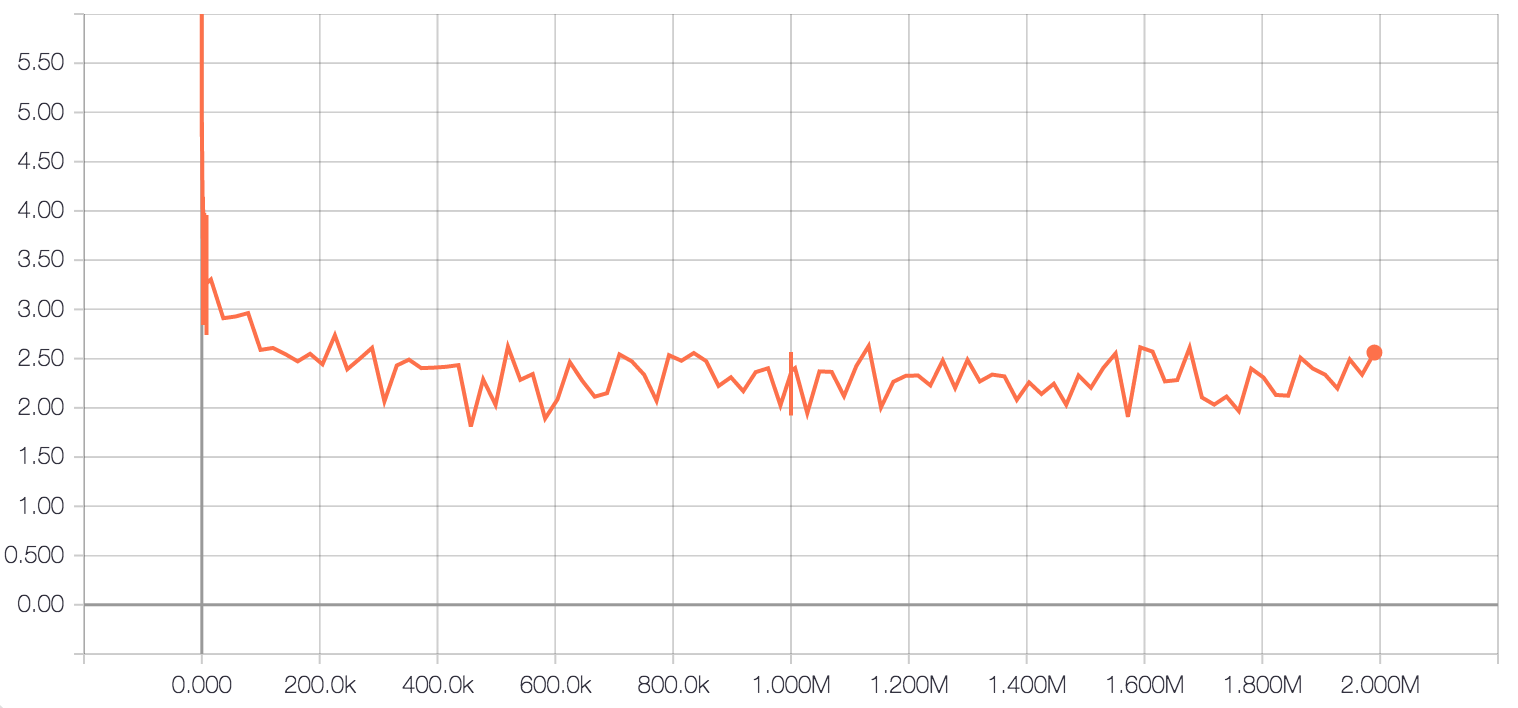
\includegraphics[width=\linewidth]{exp7-1}
  \caption{
    Función de error para el Experimento \ref{experiment:7}.
    (Fuente: elaboración propia.)
  }
  \label{exp7}
\end{figure}

\begin{experiment} \label{experiment:8}
  Con los mismos datos que para los dos experimentos anteriores y con la CNN pequeña, se realizó\
  el entrenamiento cuyo desempeño de ilustra en la Figura \ref{exp8}. Ahora se aumentó a 20 el\
  número de leyendas por imagen.
\end{experiment}

\begin{figure}[h]
  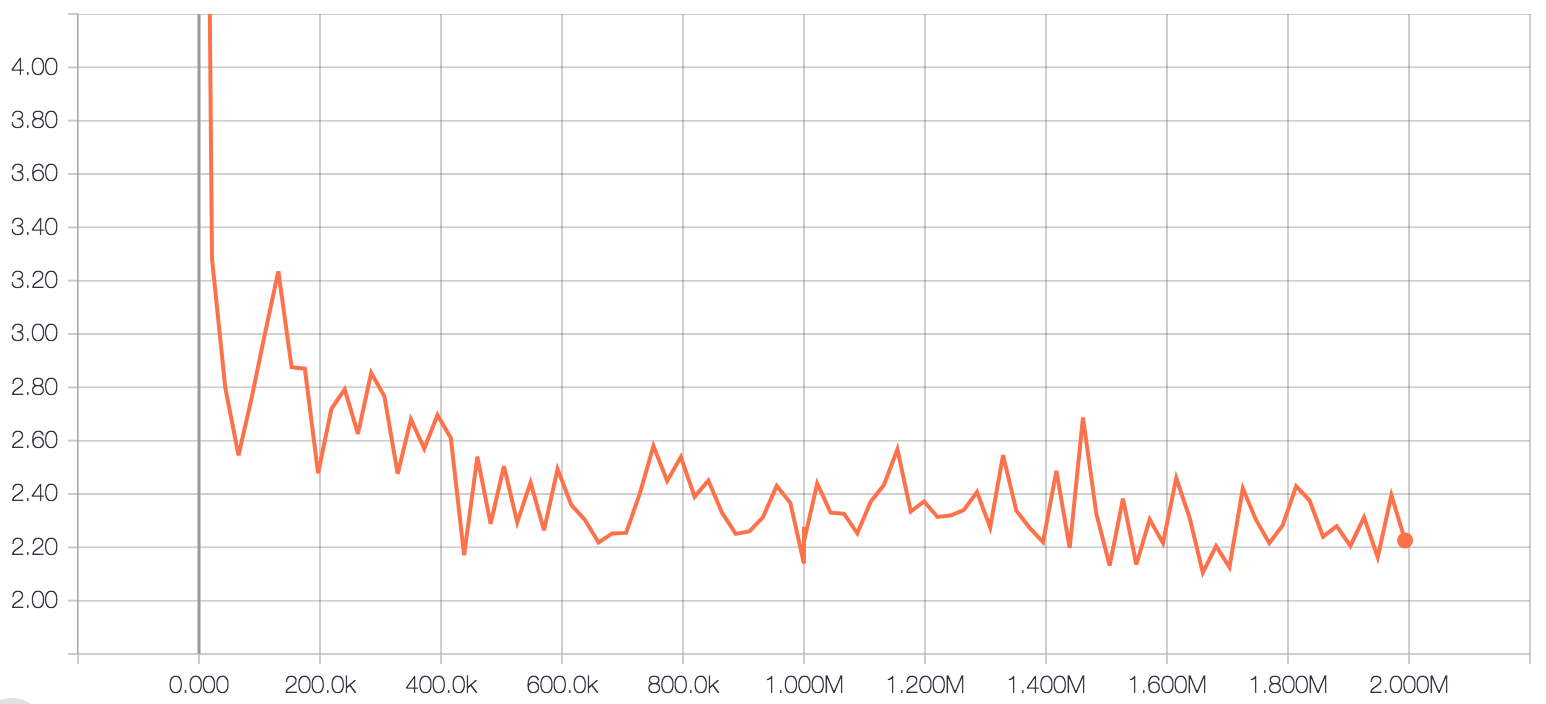
\includegraphics[width=\linewidth]{exp8-1}
  \caption{
    Función de error para el Experimento \ref{experiment:8}.
    (Fuente: elaboración propia.)
  }
  \label{exp8}
\end{figure}

\subsection{Generación de leyendas}

\noindent
El modo \verb+inferencia+ del modelo consiste en generar una leyenda para una imagen de entrada.\
Dada la manera con la cual se representa el modelo de lenguaje aprendido del conjunto de datos\
de entrenamiento, sabemos que por cada palabra hay una distribución de probabilidad que evalúa\
qué tan viable es que cada palabra del vocabulario sea la que sigue. Por lo tanto, muchas veces\
conviene observar los $k$ enunciados que \emph{mejor} describen una imagen, maximizando la\
probabilidad conjunta entre cada una de las palabras que los componen (en orden).\par
La \textbf{búsqueda por haces} (\emph{beam search}, en inglés) es algoritmo que logra calcular\
enunciados de \emph{``máxima verosimimilitud''}. El procedimiento incorpora a un agente cuyo\
objetivo es encontrar el camino de mayor \emph{peso} posible en una máquina de estados, en la cual solo\
tiene conocimiento del estado actual y los pesos para llegar a los vecinos del mismo. La salida\
del algoritmo muestra los $k$ enunciados más viables para cierta imagen. El agente, entonces\
registra de manera paralela las $k$ palabras de mayor probabilidad que sucedan a la palabra anterior.\par
Normalmente, esto se programa mediante $k$ hilos de ejecución en paralelo. Cada uno se inicializa\
aleatoriamente con las $k$ palabras de inicio de mayor probabilidad. En el paso $t$, cada\
hilo vuelve a calcular los $k$ siguientes mejores estados (un total de $k^2$ estados) y, al final,\
el agente se queda con los mejores $k$ para proceder al paso $t+1$. En este caso, se consideraron\
los $k=3$ mejores enunciados para cada imagen.

\section{Evaluación} \label{sec:metrics}

\noindent
La evaluación de un modelo de aprendizaje automático suele ser un proceso subestimado, sobre todo\
si la función de error elegida para ser optimizada fue minimizada durante el entrenamiento.\
No obstante, el efectuar algunas métricas, traen consigo evidencia de la buena generalización\
del modelo. Las Figuras \ref{eval:exp2} y \ref{eval:exp3} ilustran con gráficos algunas métricas de\
evaluación utilizadas para el desempeño de las CNNs usadas para los experimentos.

\begin{figure}[H]
  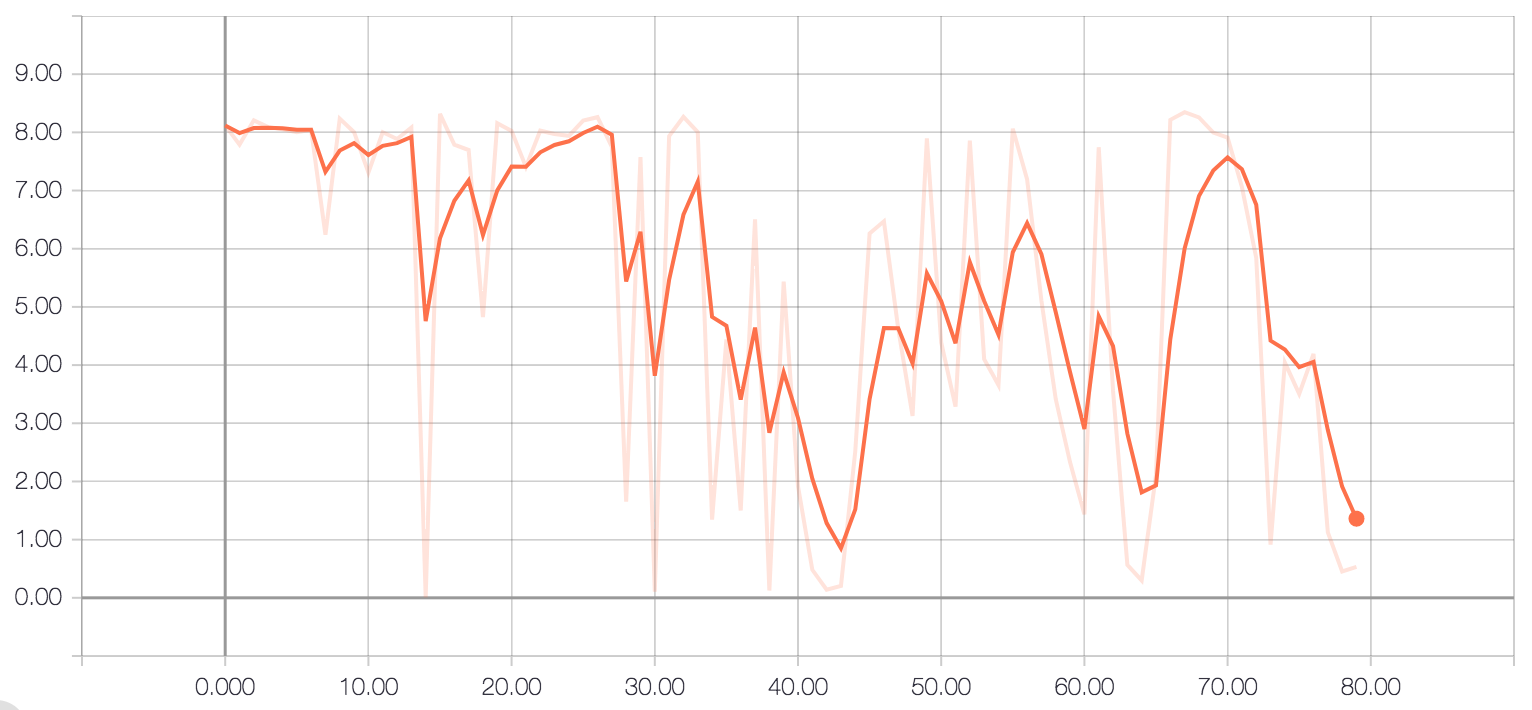
\includegraphics[width=\linewidth]{exp2-2}
  \caption[Nota al pie]{
    Función de error para el Experimento \ref{experiment:2}, en la que se
    calcula la \emph{precisión}\footnotemark del modelo con el conjunto de
    datos de entrenamiento.
    (Fuente: elaboración propia.)
  }
  \label{eval:exp2}
\end{figure}

\begin{figure}[H]
  \centering
  \begin{minipage}[c]{\linewidth}
    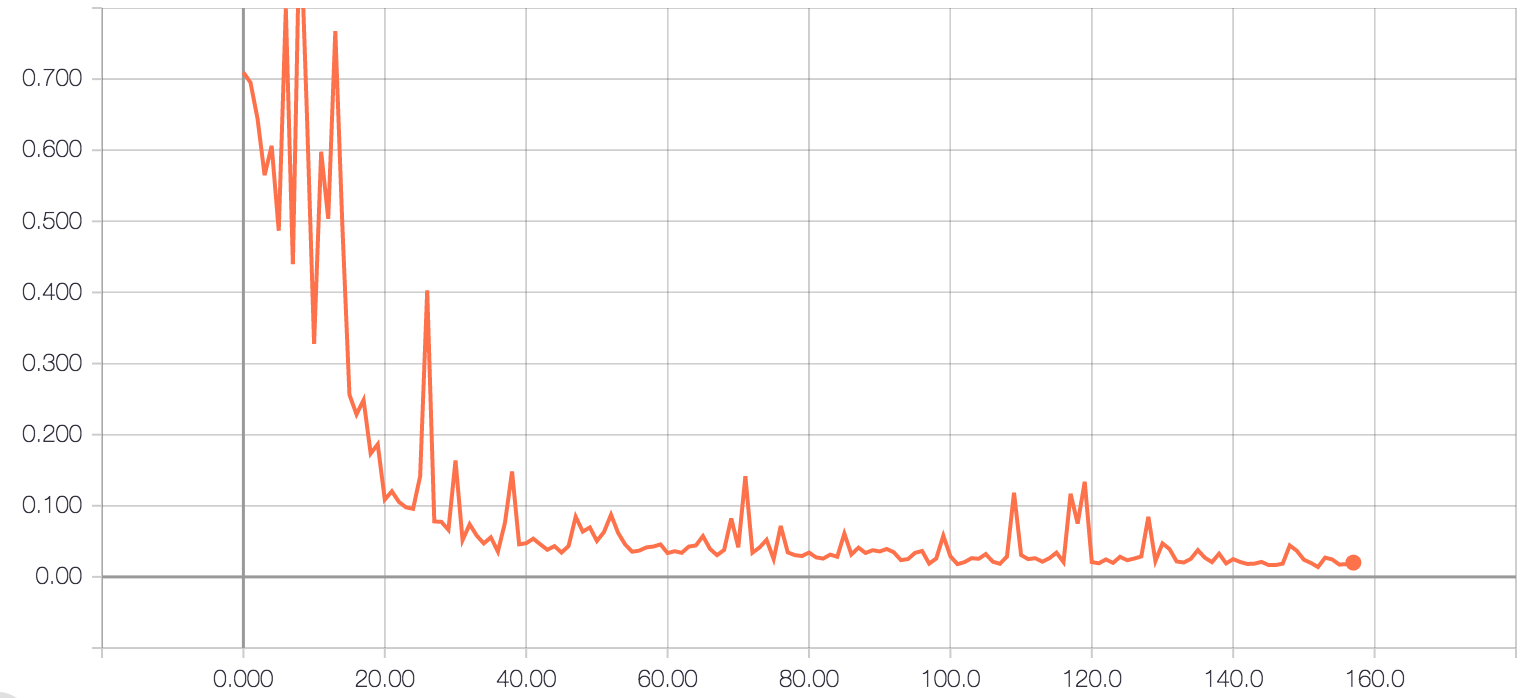
\includegraphics[width=\linewidth]{exp3-2}
  \end{minipage}\hfill
  \begin{minipage}[c]{\linewidth}
    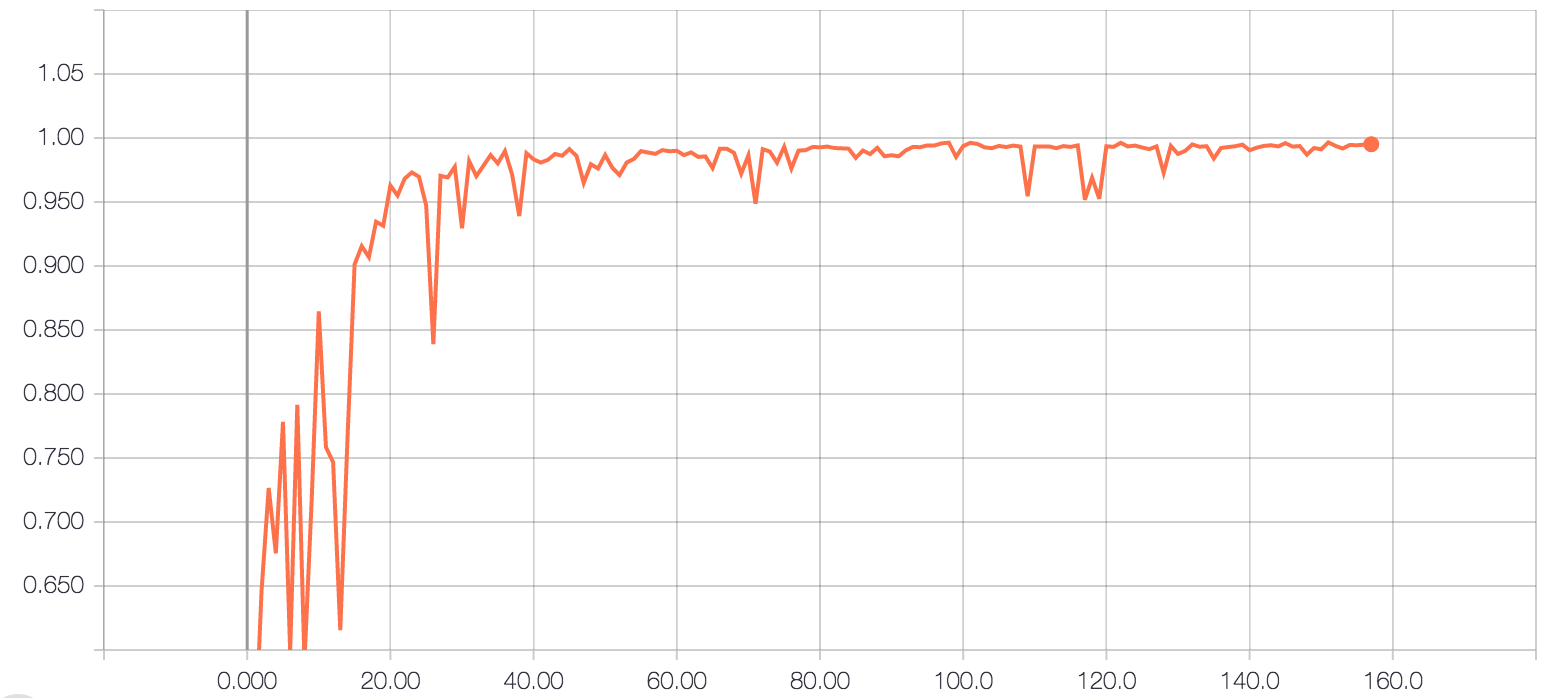
\includegraphics[width=\linewidth]{exp3-3}
  \end{minipage}
  \caption[Nota al pie]{
    Dos funciones de evaluación para el Experimento \ref{experiment:3}.
    Ambas calculan la \emph{precisión} con la que el modelo realiza
    sus clasificaciones. El gráfico de la parte superior muestra dicha métrica
    utilizando los datos de entrenamiento, mientras que para la parte inferior, se
    usaron los datos de \emph{validación}, los cuales se obtuvieron muestreando\
    aleatoriamente el $20\%$ del total de los datos para afinar la red neuronal.
    (Fuente: elaboración propia.)
  }
  \label{eval:exp3}
\end{figure}

\footnotetext{
  La \textbf{precisión} (\emph{accuracy}, en inglés) puede ser entendida como el porcentaje\
  de aciertos que tiene el modelo al intentar predecir un lote de datos. Se busca, entonces,\
  que su valor esté muy cercano a 1.
}

En el contexto del procesamiento del lenguaje natural, es común preguntarse qué tan \emph{buenos}\
son los enunciados generados con respecto a un lenguaje referencia. En este caso, se trata\
de un lenguaje informal, generado a partir de la popularidad que adquieren ciertas frases\
dentro del Internet. Sin embargo, es posible discernir entre un enunciado que hace sentido\
empírico a uno que combina palabras sin patrón alguno.\par
Las métricas sugeridas en \cite{DBLP:journals/corr/VinyalsTBE16} sugieren el uso de un corpus\
lingüístico de referencia, con el cual se compare la similitud entre las estructuras gramaticales\
generadas por el modelo con enunciados ``reales''. Debido a la dificultad en tiempos y la ambigüedad\
que puede existir para reunir dicho corpus (¡el humor de los memes está muy definido por gustos personales!),\
se prefirió reportar otro método.\par
En particular, analizamos qué tan bien aprende el modelo a predecir la $t$-ésima palabra, a nivel\
probabilístico. Dada la distribución de probabilidad $p(\cdot)$ que aprende la LSTM sobre todos\
los enunciados posibles del vocabulario, definimos la \textbf{perplejidad} $PP(S)$ del modelo,\
dado un enunciado $S = s_1 s_2 \ldots s_n$, como
\begin{align}
  PP(S) = p(s_1 s_2 \ldots s_n) ^{-\frac{1}{n}}.
\end{align}
Intuitivamente, la \emph{perplejidad} del modelo nos dice el número de posibles candidatos que tiene\
el modelo para la palabra $s_{t+1}$, dadas $s_1, s_2, \ldots, s_t$. Si la \emph{perplejidad} es minimizada,\
entonces el modelo aprende con éxito a descubrir patrones de secuencias de palabras.\par
Para el Experimento \ref{experiment:7}, reportamos una \emph{perplejidad} final de $70.2$, dado un vocabulario\
de 7413 palabras. Anteriormente, el primer experimento logra minimizar su \emph{perplejidad}\
considerablemente (Figura \ref{eval:exp1}), generando así un buen modelo de lenguaje.

\begin{figure}[h]
  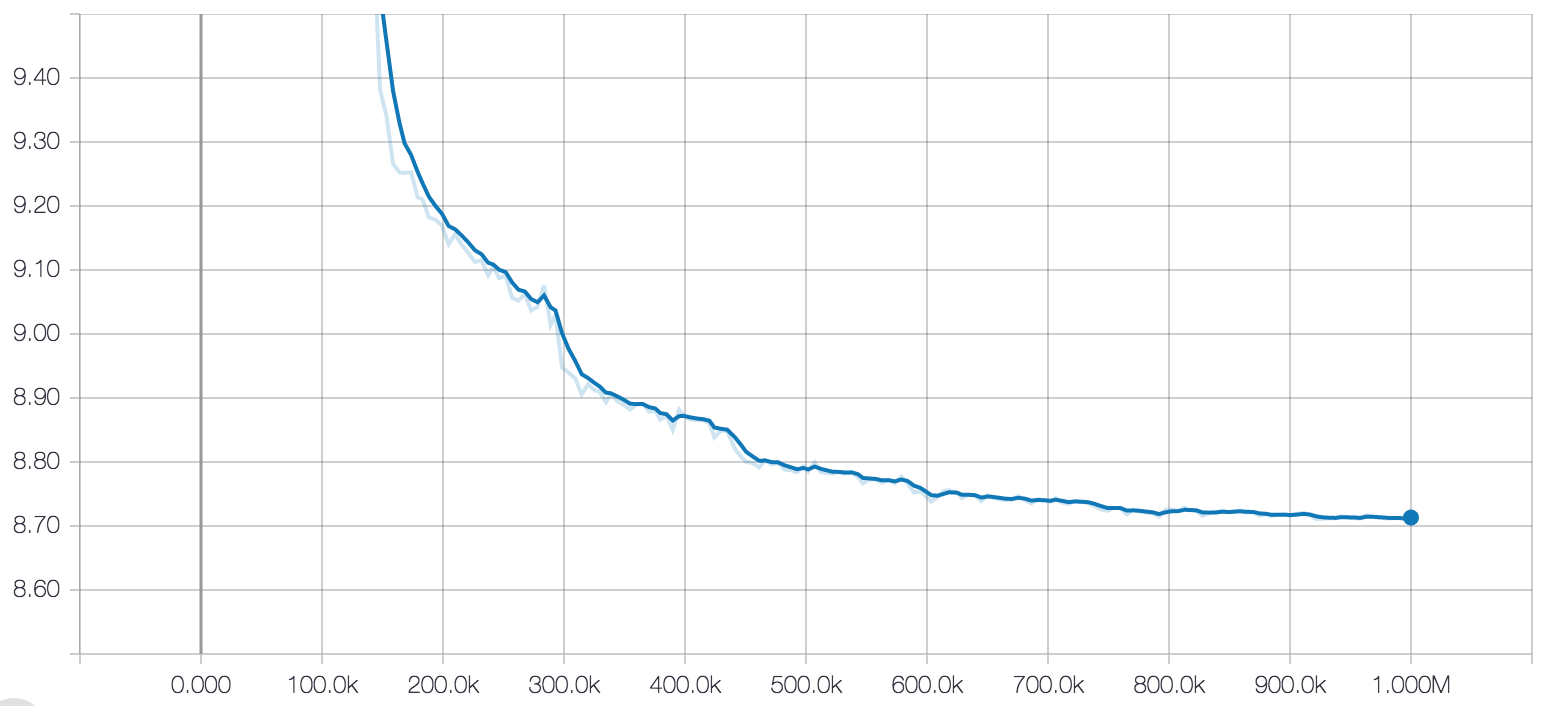
\includegraphics[width=\linewidth]{exp1-3}
  \caption{
    Minimización de la \emph{perplejidad} en el Experimento \ref{experiment:1}.
    (Fuente: elaboración propia.)
  }
  \label{eval:exp1}
\end{figure}
